%!TEX root = ../thesis.tex
%*******************************************************************************
%****************************** Third Chapter **********************************
%*******************************************************************************
\chapter{Discussion}

% **************************** Define Graphics Path **************************
\ifpdf
    \graphicspath{{Chapter4/Figs/Raster/}{Chapter4/Figs/PDF/}{Chapter4/Figs/}}
\else
    \graphicspath{{Chapter4/Figs/Vector/}{Chapter4/Figs/}}
\fi

\section{Summary of findings}

% In chapter 1 \section{}, I describe challenges and solutions associated with somatic mutation detection in bulk normal tissue. I also introduce single-molecule real-time (SMRT) sequencing from Pacific Biosciences and summarise the applications of long-read sequencing. Additionally, I describe the new opportunities presented by publicly available reference genomes and CCS reads produced by the Darwin Tree of Life (DToL) project.  

In chapter 1, I describe challenges and solutions associated with somatic mutation detection in bulk normal tissue. I also introduce single-molecule real-time (SMRT) sequencing from Pacific Biosciences and summarise the applications of long-read sequencing. Additionally, I describe the new opportunities presented by publicly available reference genomes and CCS reads produced by the Darwin Tree of Life (DToL) project.  

% In chapter 2 \section{}, I describe short-read sequencing methods that leverage redundant sequencing of the same molecule to generate highly accurate consensus sequences and their uses in detection of somatic mutations with low variant allele frequency (VAF). I hypothesise that CCS sequencing, a long-read sequencing method that takes advantage of multiple-pass sequencing of a single-molecule, has the potential to generate reads with one of the highest base accuracies among commercially available sequencing platforms. To test the hypothesis, I sequence positive control samples with characterised mutational processes and estimated mutation burdens and negative control sample with few somatic mutations. I develop himut (high-fidelity mutation) to leverage CCS read length and base accuracy for single-molecule somatic mutation detection. I also determine the limit of detection using the negative control and demonstrate that CCS bases have sufficient base accuracy to enable profiling of ongoing somatic mutational processes in human samples.

In chapter 2, I describe short-read sequencing methods that leverage redundant sequencing of the same molecule to generate highly accurate consensus sequences and their uses in detection of somatic mutations with low variant allele frequency (VAF). I hypothesise that CCS sequencing, a long-read sequencing method that takes advantage of multiple-pass sequencing of a single-molecule, has the potential to generate reads with one of the highest base accuracies among commercially available sequencing platforms. To test the hypothesis, I sequence positive control samples with characterised mutational processes and estimated mutation burdens and negative control sample with few somatic mutations. I develop himut (high-fidelity mutation) to leverage CCS read length and base accuracy for single-molecule somatic mutation detection. I also determine the limit of detection using the negative control and demonstrate that CCS bases have sufficient base accuracy to enable profiling of ongoing somatic mutational processes in human samples. 

% In Chapter 3 \section{}, I use CCS reads and high-quality reference genomes from a range of eukaryotic species publicly available through the DToL project to study germline and somatic mutational processes across the Tree of Life. To date, the cost and challenges associated with constructing high-quality reference genomes have limited the study of germline and somatic mutations to \textit{Homo sapiens} and model organisms such as \textit{Caenorhabditis elegans} \cite{Meier2014-do} and \textit{Mus musculus} \cite{}. To my knowledge, this PhD thesis is the first to discover and analyse germline and somatic mutational processes across the Tree of Life.  

In chapter 3, I use CCS reads and high-quality reference genomes from a range of eukaryotic species publicly available through the DToL project to study germline and somatic mutational processes across the Tree of Life. To date, the cost and challenges associated with constructing high-quality reference genomes have limited the study of germline and somatic mutations to \textit{Homo sapiens} and model organisms such as \textit{Caenorhabditis elegans} \cite{Meier2014-do} and \textit{Mus musculus} \cite{}. To my knowledge, this PhD thesis is the first to discover and analyse germline and somatic mutational processes across the Tree of Life.  

To support my extraordinary claim, I collected evidence to support that my method can confidently call single-molecule somatic mutations in non-human samples. The acquisition of somatic mutation begins with fertilisation, and the number of accrued somatic mutations increase with time.  I collected, sequenced and detected somatic mutations in \textit{Phorcus lineatus} samples of various ages (3, 5 and 15). \textit{P. lineatus} mutation burden, total number of somatic mutations per cell, increased with age, demonstrating that CCS reads can be also used to call somatic mutations in non-human samples. In addition, I confirmed that the unique mutational spectrum observed in each species is due to biological processes rather than stochastic processes in the experimental design by sequencing multiple samples from a subset of species and independently observing the same mutational spectrum. 

Armed with confidence in himut's ability to call somatic mutations in bulk tissues from non-human samples, I used deepvariant and himut to detect germline and somatic mutations in \textit{603} samples from \textit{597} eukaryotic species and extracted 21 germline and 85 somatic mutational signatures. The high cosine similarity between germline and somatic mutational signatures also bolstered my confidence in the results. I performed phylogenetic analysis to not only identify mutational signatures that are shared between samples based on their common ancestor, habitat, and taxonomic classification. 

\section{Limitations}

\subsection{CCS library, sequencing and consensus sequence generation errors}

Currently, the CCS library preparation protocol is not designed to minimise the introduction of duplex library errors or to correctly repair these errors. In addition, the consensus sequence generation algorithm is not optimised to produce CCS reads with bases assigned correct base-specific error probabilities. Consequently, I limited somatic mutation detection to Q93 CCS bases, assuming that the generation of Q93 CCS bases from library and sequencing errors is improbable. In theory, multiple subreads with the same error on both strands of the DNA would be required to produce CCS bases with high quality values. However, in practice, duplex library errors can alter both strands of the DNA and context specific sequencing error can independently generate the same error across all the subreads from the same ZMW.  

In chapter 2, I used CCS reads from normal cord blood granulocytes with few somatic mutations to measure the base accuracy of Q93 CCS bases. I estimate the Q93 CCS substitution error rate to range from Q60 to Q90, depending on the substitution and the trinucleotide context. More importantly, I show that false positive substitutions are derived from inaccurate BQ score estimates and that more accurate BQ score estimates are obtainable from the underlying sequence data. Hence, the current SMRT sequencing capabilities are not a limiting factor to the generation of more accurate CCS bases. 

% In chapter 2 \section{}, I used CCS reads from normal cord blood granulocytes with few somatic mutations to measure the base accuracy of Q93 CCS bases. I estimate the Q93 CCS substitution error rate to range from Q60 to Q90, depending on the substitution and the trinucleotide context. More importantly, I show that false positive substitutions are derived from inaccurate BQ score estimates and that more accurate BQ score estimates are obtainable from the underlying sequence data. Hence, the current SMRT sequencing capabilities are not a limiting factor to the generation of more accurate CCS bases. 

In chapter 3, I used himut to detect somatic mutations from bulk normal tissue in a range of eukaryotic species and performed mutational signature analysis to extract novel germline and somatic mutational signatures across the Tree of Life. In the process, I also identified three artefactual mutational signatures: one from library error and two from sequencing errors. Samples exhibiting an artefactual signature associated with library errors showed a somatic mutational spectrum inconsistent with the germline mutational spectrum and a highly elevated mutation burden compared to samples from the same taxonomic classification. 

\subsection{Single-molecule somatic mutation detection}

In chapter 2 and 3, I demonstrate that CCS bases have sufficient base accuracy to profile ongoing somatic mutational processes from bulk normal tissue, agnostic of species and clonality. Currently, CCS reads have higher sequencing error rate than nanorate duplex reads. Consequently, himut cannot ascertain whether an individual substitution, where a single read supports the mismatch between the read and the reference genome, is an error or a somatic mutation. In the distant future, consensus sequence generation algorithm could generate CCS reads with more accurate bases and base accuracy estimates to improve somatic mutation detection sensitivity. In the immediate future, knowledge of active mutational processes within each tissue could be leveraged to determine the likelihood that the observed mismatch originates from a biological process or from an error process.

Multiple mutational processes act on the genome at any given time, and they can generate identical mutations within the same sequence context. Given a catalogue of somatic mutations from multiple samples, mutational signature analysis is performed to identify the mutational signature observed in each sample and the contribution of each mutational signature to the mutation burden of the sample (equation \ref{eq:1}). Each mutational signature represents a biological process and reflects the probability that the biological process will generate a somatic mutation in a specific sequence context 

\begin{align}
\begin{split} 
M &\approx PE \label{eq:1} \\
\begin{bmatrix}
    m^{1}_{1} & \dots & m^{1}_{j} \\
    \vdots & \ddots & \vdots \\
    m^{96}_{1} & \dots & m^{96}_{j} \\
\end{bmatrix} &\approx
\begin{bmatrix}
    p^{1}_{1} & \dots & p^{1}_{s} \\
    \vdots & \ddots & \vdots \\
    p^{96}_{1} & \dots & p^{96}_{s} \\
\end{bmatrix} \times
\begin{bmatrix}
    e^{1}_{1} & \dots & e^{s}_{j} \\
    \vdots & \ddots & \vdots \\
    e^{s}_{1} & \dots & e^{s}_{j} \\
\end{bmatrix} 
\end{split}
\end{align}

where $M$ is the somatic mutation catalogue matrix with mutation type as rows and samples as columns. $P$ is the mutational signature matrix with mutation types as rows and signatures as columns. $E$ is the exposure matrix with signatures as rows and samples as columns. Here, I use the mutation types as defined by the SBS96 classification system, where substitution in the pyrimidine context is further classified based on the trinucleotide context, for this example.

Typically, mutational signature analysis ends with the identification of new somatic mutational processes, if any exist, and the attribution of known mutational signatures to the mutation burden of each sample. However, mutational signature analysis can also be extended to calculate the posterior probability that an individual somatic mutation originated from a specific mutational signature, given the mutational signatures identified in the sample of interest (equation \ref{eq:2}). This method was previously used to determine the SBS16 mutational signature, a signature associated with alcohol consumption, as the main source of somatic mutations in the CTNNB1 gene in hepatocellular carcinoma \cite{Letouze2017-tl}. 

\begin{equation} \label{eq:2} 
P(m,s) = \frac{p^{i}_{s} \times e^{s}_{j}}{\sum^{n}_{s=1}p^{i}_{s} \times e^{s}_{j}}
\end{equation}

Before the improvement of CCS base accuracy and BQ score estimates, the above method could potentially be employed to calculate the posterior probability that an individual somatic mutation is derived from a biological process or a sequencing error. Thereafter, these posterior probabilities serve as a proxy for confidence in somatic mutation detection.

\section{Discussion}

\subsection{Public health}

The All of Us (AoU) research program aims to sequence the genomes and collect electronic health records (EHR) data of at least one million individuals in the United States from under-represented demographic categories to accelerate biomedical research \cite{AoU2019}. In a manner similar to my use of himut for somatic mutational processes within the Tree of Life, the AoU research program can potentially use himut to investigate somatic mutagenesis in all their samples where CCS reads are available. The number of samples sequenced under the AoU research program will enable the discovery of new mutational signatures resulting from environmental mutagenesis, DNA damage repair deficiencies, as well as their possible combinations. Moreover, the AoU research program can also leverage the EHR records (e.g., age of the sample, geographical location, dietary and drinking habits, and drug prescription history) to develop and evaluate hypotheses about the aetiology of the newly discovered mutational signatures.

The tobacco smoking mutational signature (SBS4) is a canonical example of a mutational signature where exogenous exposure to a mutagen (tobacco carcinogen) is responsible for newly acquired somatic mutations. The higher mutation burden attributable to SBS4 in smokers compared to non-smokers indicates that tobacco smoking increases the risk of lung cancer \cite{Alexandrov2016-uw}. In addition, aristolochic acid (AA) consumption introduces T>A somatic mutations (SBS22) and is a major contributor to endemic Balkan nephropathy \cite{Grollman2007-rh} and urinary tract urothelial carcinoma in Taiwan \cite{Chen2012-vh}. The identification of new mutagens and discovery of new somatic mutational signatures might be one of the most intriguing outcomes of future population-scale sequencing efforts. 


\subsection{DNA forensics}

DNA fingerprinting is often used in criminal investigations to determine whether the reference DNA sample from the crime scene and the DNA sample from the suspect are derived from the same individual \cite{Gill1985-dt}. If the genetic sequences of two random individuals are compared, 99.9\% of their genetic sequences are estimated to be identical \cite{1000_Genomes_Project_Consortium2012-rj}. However, the number of core repeat motifs in variable number tandem repeat (VNTR) loci is unique to everyone. DNA fingerprinting leverages this variation in VNTR loci as a biomarker to compare DNA samples from different individuals for paternity testing and forensic analysis.  

The age of the sample is another biomarker that can function as an identifier.  Typically, cells accrue somatic mutations at a constant rate. For example, haematopoietic stem cells acquire 16.8 substitutions per cell per year \cite{Mitchell2022-ry, Osorio2018-mh} while sperm cells with the lowest somatic mutation rate accumulate 2.9 substitutions per cell per year \cite{Rahbari2016-ot}. Hence, if the tissue type of the DNA sample is known, age of the sample can be calculated from the mutation burden and the tissue-specific somatic mutation rate. In the future, himut can be potentially used to identify the age of the sample at the date of collection, thereby provide incriminating evidence or exonerating innocent individuals. 

\subsection{Germline and somatic mutational processes across the Tree of Life}

Every living species on Earth is thought to be the direct descendent of the last universal common ancestor (LUCA). The Tree of Life symbolises how different species share a common ancestor and how they have diverged over time through speciation and natural selection. Somatic mutagenesis in parental cells of asexually reproducing species or gametes of sexually reproducing species is at the heart of evolution as somatic mutational processes generate the genetic diversity that natural and sexual selection act upon for adaptation and speciation. Using CCS reads and high-quality reference genomes from the DToL project, I had the privilege to detect, analyse and discover new and conserved somatic mutational processes across the Tree of Life and time the emergence of these somatic mutational processes. 

In many eukaryotic species, the same somatic mutational process is responsible for generating mutations in both gametes and somatic cells, but in a subset of species such as the \textit{P. albimanus} (white-footed hoverfly) and \textit{S. pipiens} (thicked-legged hoverfly) somatic mutational process of an unknown aetiology is not only distinct from the germline mutational processes, but also exhibits transcriptional-strand bias. The presence of the same somatic mutational process in biological replicates confirms that the observed mutational signature is a consequence of a specific biological process. 

The presence of SBS1 mutational signature in the Animal, Fungi and Plant kingdom underscores the importance of cytosine methylation as an epigenetic mechanism. In \textit{C. elegans}, the loss of DNA methyltransferase 1 (DNMT1), a drastic measure, is required to eliminate cytosine methylation and subsequent deamination of 5mC to thymine. 

The discovery of a greater number of unique somatic mutational processes in the insect phylum, compared to other phyla, is another unexpected revelation. The insect phylum boasts the greatest diversity among all phyla in the Animal kingdom not only in the number of individuals, but also the number of species. The greater diversity of somatic mutational processes is presumably linked to the successful adaptation and speciation of insect phylum in ecological niches where other phyla have been unsuccessful. The absence of additional somatic mutational processes that act upon the gametes in other phyla of the animal kingdom suggests that other somatic mutational processes have a selective disadvantage to the individual. If this is indeed true, a natural question arises: why are new somatic mutational processes harmful to individuals of non-insect phyla, and what properties have allowed SBS1 mutational signature to be conserved across so many species for billions of years? Furthermore, how has the insect phylum evolved not just one new somatic mutational process, but multiple new processes? And how has the DNA damage pathway evolved to accommodate the dramatic changes in somatic mutational process that occur during speciation? 

\subsection{Evolutionary advantage of complete metamorphosis}

Coleoptera, Hymenoptera, Diptera and Lepidoptra, insects that undergo complete metamorphosis, account for more than 80\% of known insect species and 95\% of total insect species diversity (Figure \ref{figure:papilo-machaon}). Many theories have been proposed to explain the evolutionary advantage of complete metamorphosis such as the decoupling of growth and differentiation \cite{Rolff2019-ef}, the ability to exploit different environments \cite{Darwin1859}, and reduction in competition between juvenile insect and adult insect for limited resources \cite{Ebenman1992-in}. Here, I hypothesise that the complete metamorphosis decouples the somatic mutations acquired in the juvenile stage with that acquired in the adult stage. 

\begin{figure}[h!]
\caption{The life cycle of a \textit{Papilo machaon}}
\label{figure:papilo-machaon}
\begin{centering}
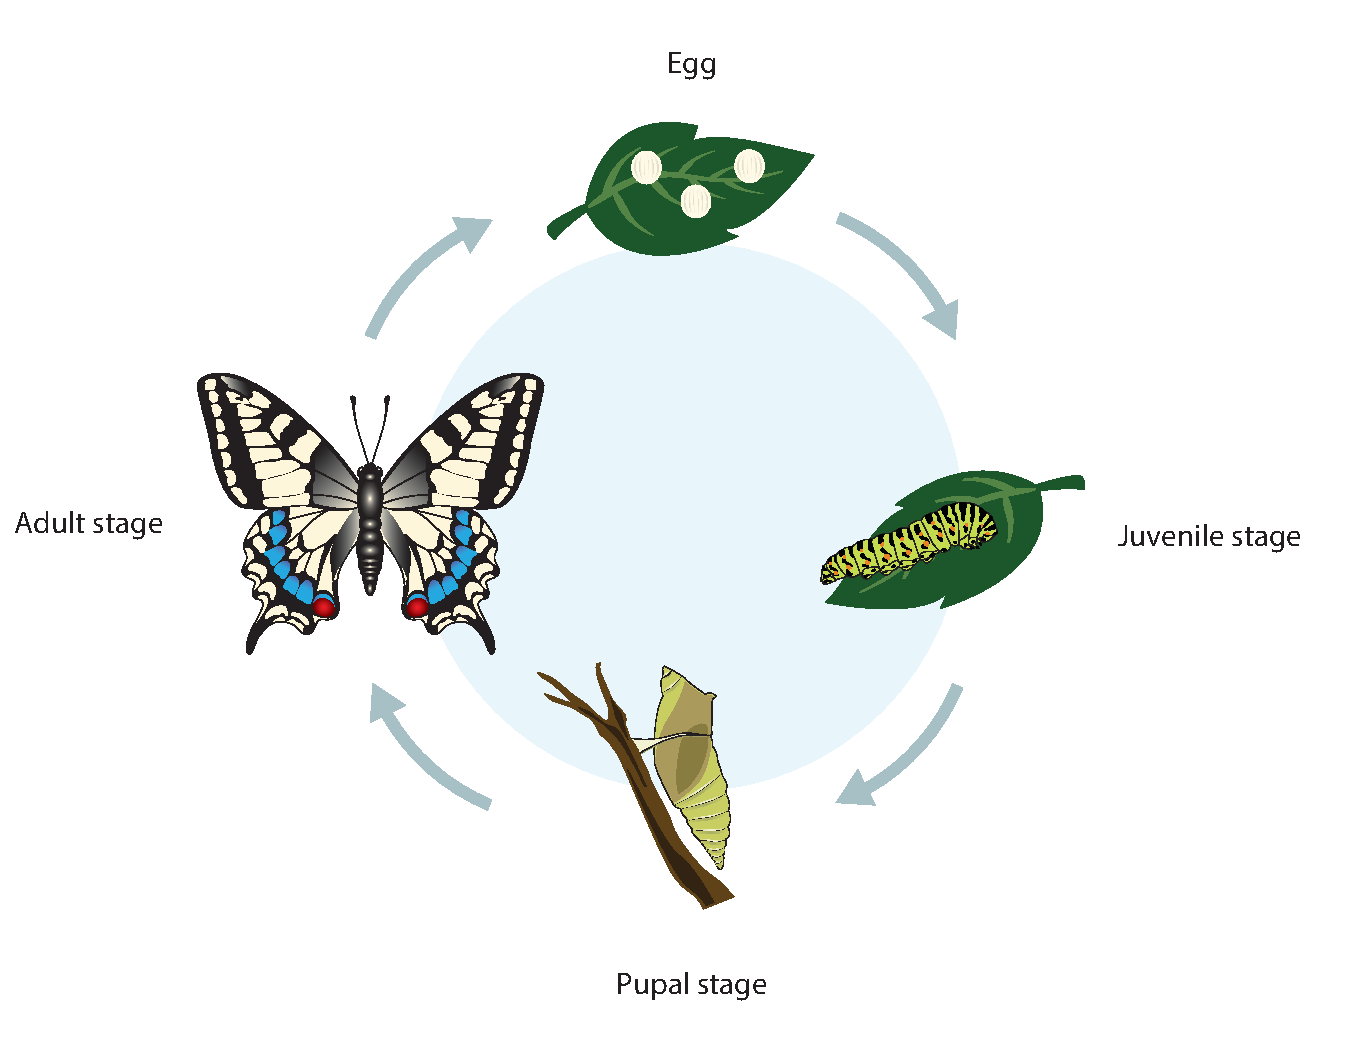
\includegraphics[width=0.9\textwidth]{papilo_machaon_life_cycle.pdf} 
\end{centering}
\end{figure}

The somatic mutation theory of ageing suggests that the gradual accumulation of somatic mutations leads to a decline in cellular function, which ultimately contributes to the ageing process \cite{Szilard1959-ru}. The theory also implies that shorter-lived species will have a higher somatic mutation rate than longer-lived species. Since somatic mutation rate is inversely proportional to the lifespan of species in mammals \cite{Cagan2022-yn}, I initially conjectured that somatic mutation rate would be higher in insects as most insects are short-lived \cite{Promislow2022-en}. However, I observed that mutation burden of insects was lower than what might have been expected from the somatic mutation theory of ageing. An alternative explanation was required for this observation (Here, I would like to highlight again that the calculation of somatic mutation rate was not within the scope of this study and requires the sequencing of multiple samples of different ages. Currently, the DToL project sequences one sample per species and age of the sample is often not recorded). 

The dichotomy in human germline and somatic mutation rates and mutational processes demonstrates the importance of mechanisms evolved to maintain the integrity of the germline genome. For example, the human oogonia and spermatogonia have the lowest mutation rates among human tissue \cite{Rahbari2016-ot}. In contrast, as a disposable tissue that does not contribute to the germline lineage, the human placenta has a higher mutation burden and chromosomal alterations that are absent in the foetus \cite{Coorens2021-ct}. This observation 

Similarly, in holometabola (a superorder of insects that undergo complete metamorphosis) larval tissue is disposable, contributing neither to adult development, nor to the transmission of genetic information to the next generation. To separate the stem cells contributing to larval development from those contributing to adult development, imaginal discs – single layers of epithelial sheets with 20 to 40 cells that develop into adult tissue during the pupal stage – are set apart from embryonic stem cells that differentiate into larval tissue early in embryonic development \cite{Wieschaus1976}. For example, genitalia are derived from the medial disc in \textit{D. melanogaster} \cite{Bate1993}. Thus, larval and adult insects are derived from distinct embryonic lineages, with the exception of the histoblast cells that develop into the abdomen of the adult insect \cite{Bate1993}. Consequently, in theory, somatic mutations acquired in the larval stage should be absent in the adult insect, and only the mosaic mutations that arose during the first few cell divisions of embryonic development should be shared between the two stages (Figure \ref{figure:lepidoptera-mutation-burden}). 

For example, caterpillars, the larvae of butterflies and moths, primarily consume leaves, stems, and flowers of plants, and the subsequent accumulation of chlorophyll pigment might be phototoxic to caterpillars. During photosynthesis, the photoexcitation of chlorophyll pigment is channelled to convert light energy into glucose and oxygen. Conversely, unregulated photoexcitation of chlorophyll pigment can produce greater quantities of reactive oxygen species in the internal organs of larvae \cite{Foyer2018-in}. Here, I hypothesise that N[C>A]A and N[C>A]T somatic mutations, linked to DNA damage from reactive oxygen species (SBS18 and SBS36), could be the primary source of somatic mutations in caterpillars, and that these somatic mutations are not transmitted to adult tissue.  


\begin{figure}[h!]
\caption{Hypothetical changes in mutation burden with life cycle progression}
\label{figure:lepidoptera-mutation-burden}
\begin{centering}
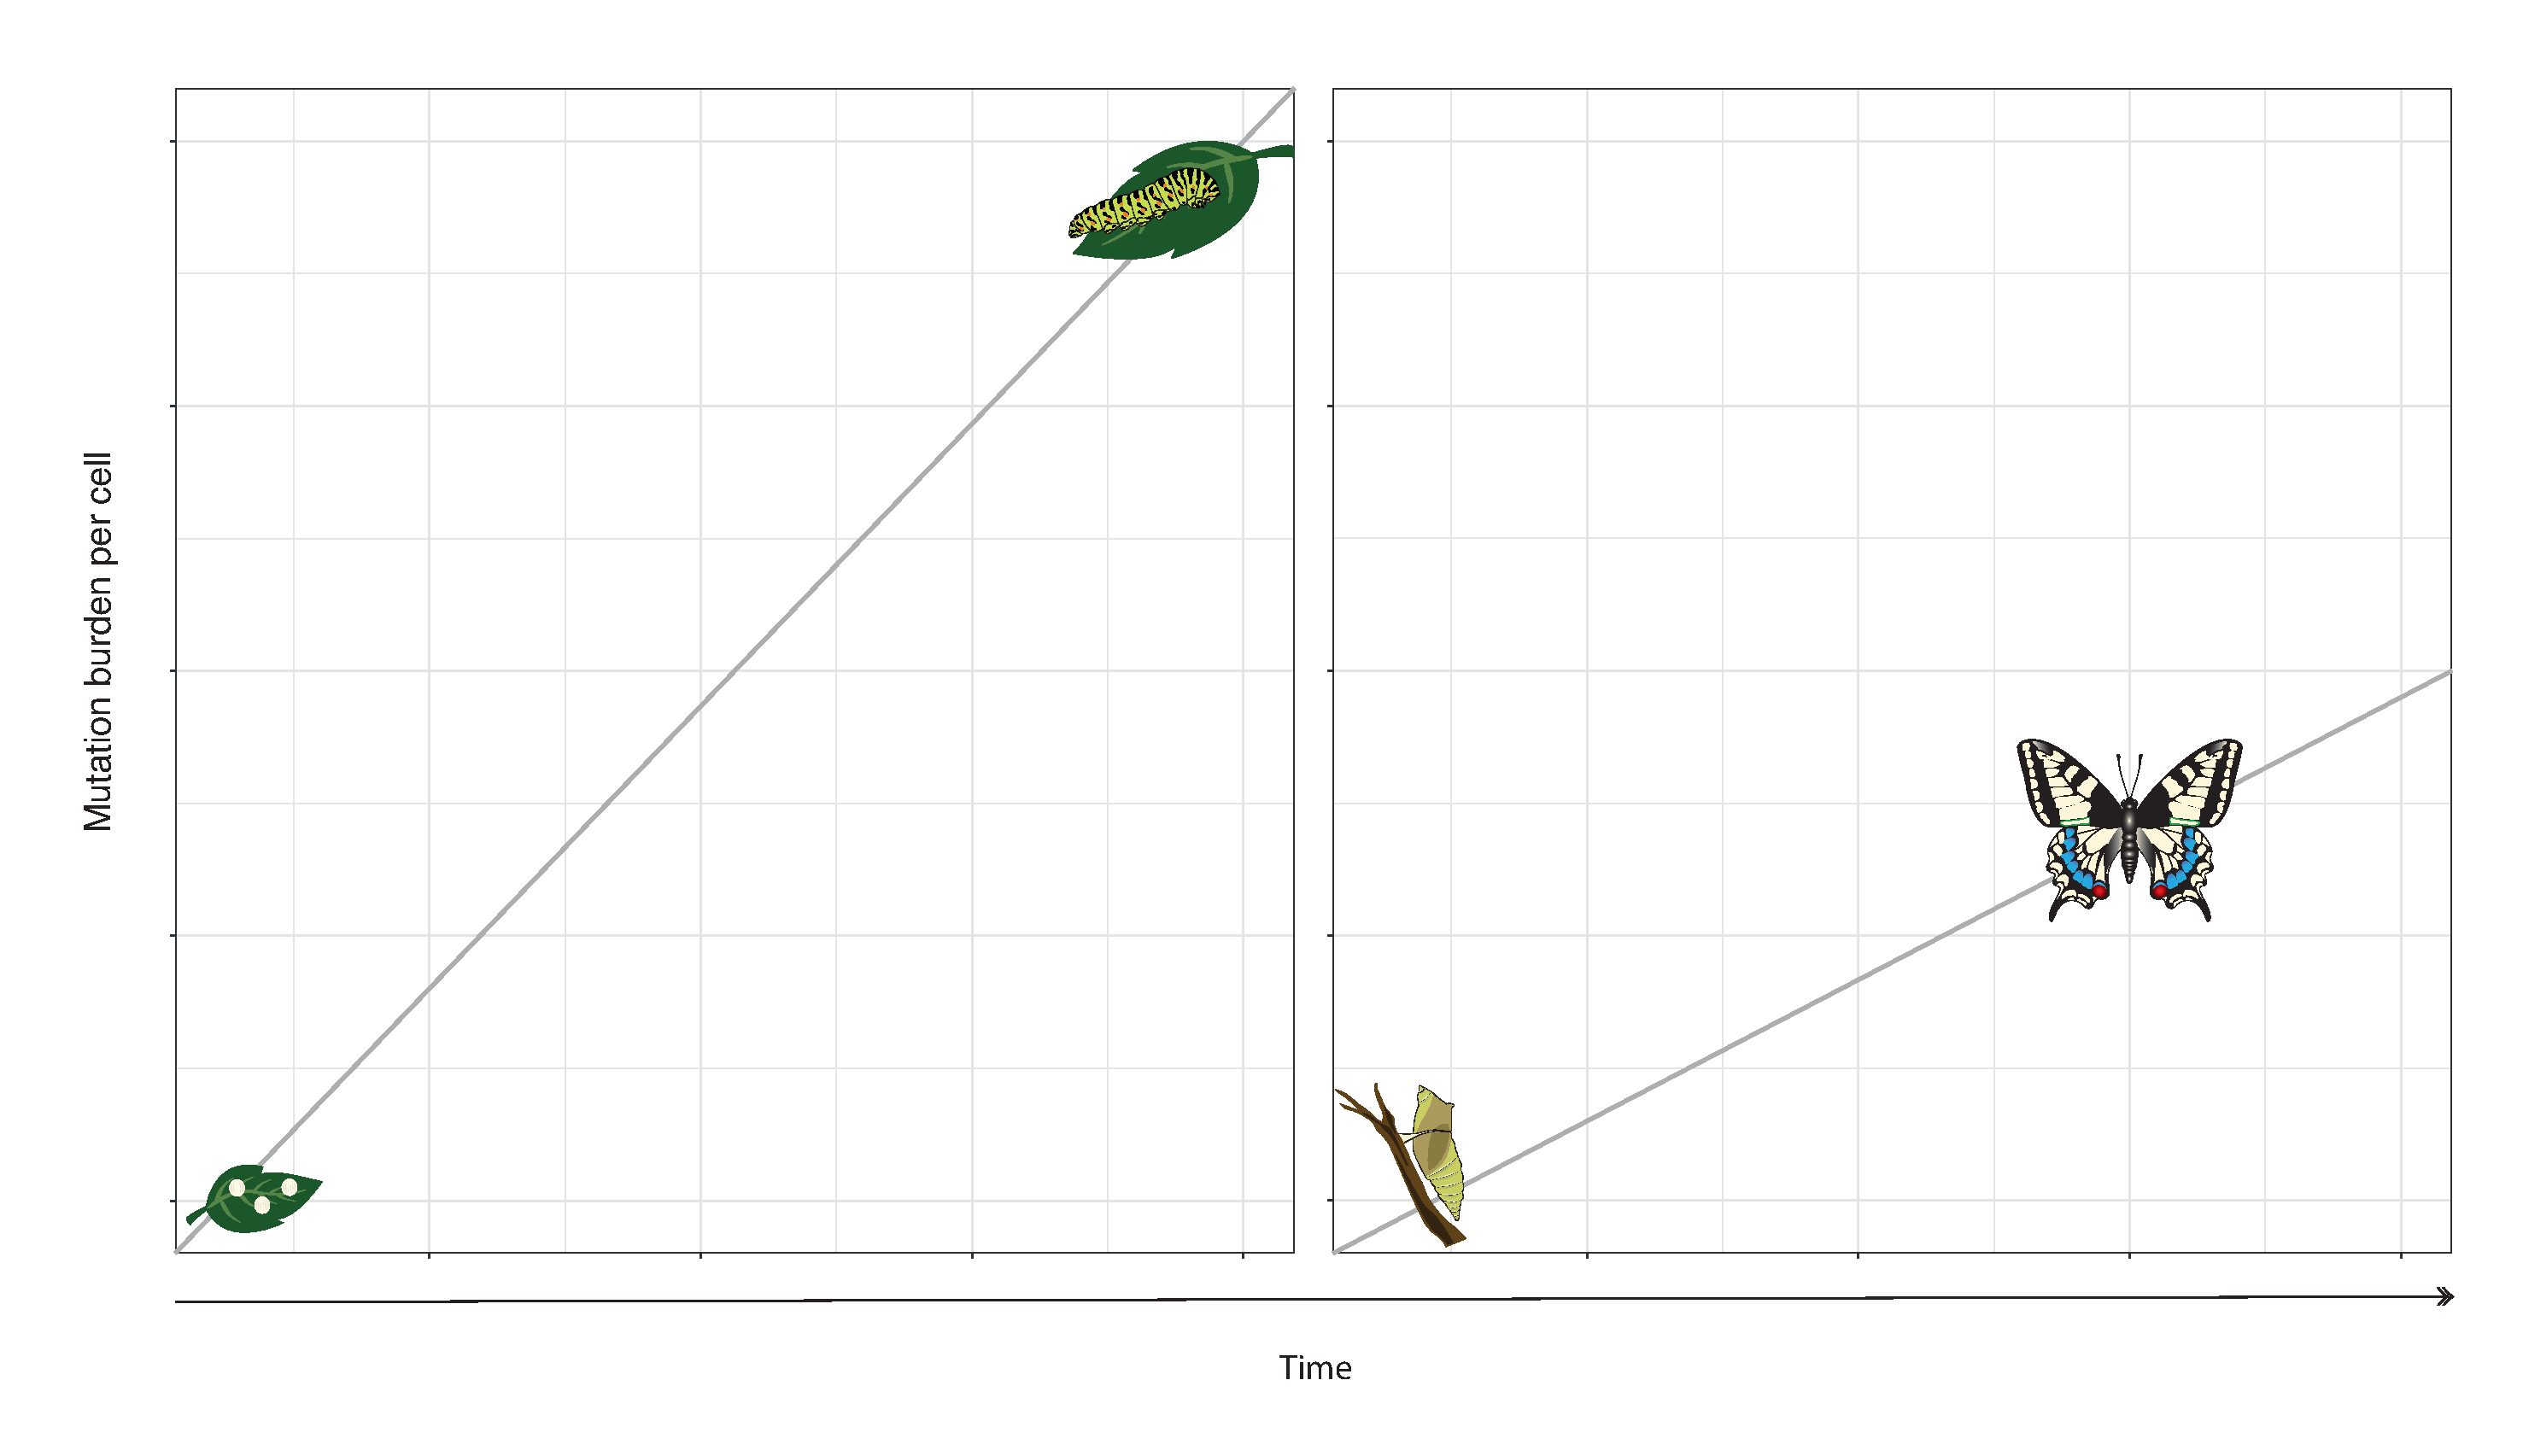
\includegraphics[width=\textwidth]{lepidoptera_mutation_burden.pdf} 
\end{centering}
\floatfoot{Larval tissue is hypothesised to have a higher somatic mutation rate than adult tissue. Somatic mutations acquired during the juvenile stage are not transmitted to the adult insect and a new somatic mutational process is operational in the adult tissue. }
\end{figure}

The life cycle and development of holometabolous insects corroborates the hypothesis that somatic mutations acquired during the larval stage are not shared with the adult insect. This hypothesis can potentially be tested with insect species that exhibit sexual dimorphism in development. In certain insect species, females do not undergo metamorphosis, and are referred to as larviform females, while the males still undergo complete metamorphosis. If the hypothesis is the correct, female samples of the same age group will exhibit a higher mutation burden than their male counterparts. CCS sequencing of multiple tissues from both male and female samples exhibiting sexual dimorphism, with known ages across multiple species, could confirm whether larval tissue indeed has a higher somatic mutation rate than adult tissue and whether somatic mutations acquired during the juvenile stage are not transmitted to the adult tissue. 

\section{Future directions}

In the imminent future, I conjecture that CCS library preparation errors and inaccurate CCS BQ score estimation will be properly addressed, and that the majority (>50\%) of CCS bases will have approximately $\sim$Q90 base accuracy. Here, I discuss the potential opportunities following this development.

\subsection{Single-molecule real-time sequencing}

As discussed in Chapter 1, CCS sequence throughput and per-base sequencing cost are functions of the number of ZMWs and the read-of-insert length of the SMRTbell template. As demonstrated in Chapter 2 and Chapter 3, CCS base accuracy is a function of subread error rate and the number of subreads used to generate the CCS read. Here, I make future predictions about forthcoming advancements in the SMRT sequencing platform based on the observations made in this PhD thesis. 

I expect the number of ZMWs per SMRTcell to double every two to three years, similar to how the number of transistors per chip doubles approximately every two years. As the number of ZMWs per SMRTcell increases exponentially, per-base sequencing cost is expected to decrease exponentially as well (Fig \ref{figure:ccs_sequence_throughput}a). Moore’s law has continued for $\sim$50 years, and similar progress is expected from SMRTcell development as well. Strikingly, read-of-insert length has increased 20-fold from 1kb to 20kb. The rate at which CCS sequence throughput increases could exceed our expectations, with the increase in both CCS read length and the number of ZMWs per SMRTcell (Fig \ref{figure:ccs_sequence_throughput}b). 


\begin{figure}[h]
\caption{Exponential decay in CCS sequencing cost}\label{figure:ccs_sequence_throughput}
\begin{centering}
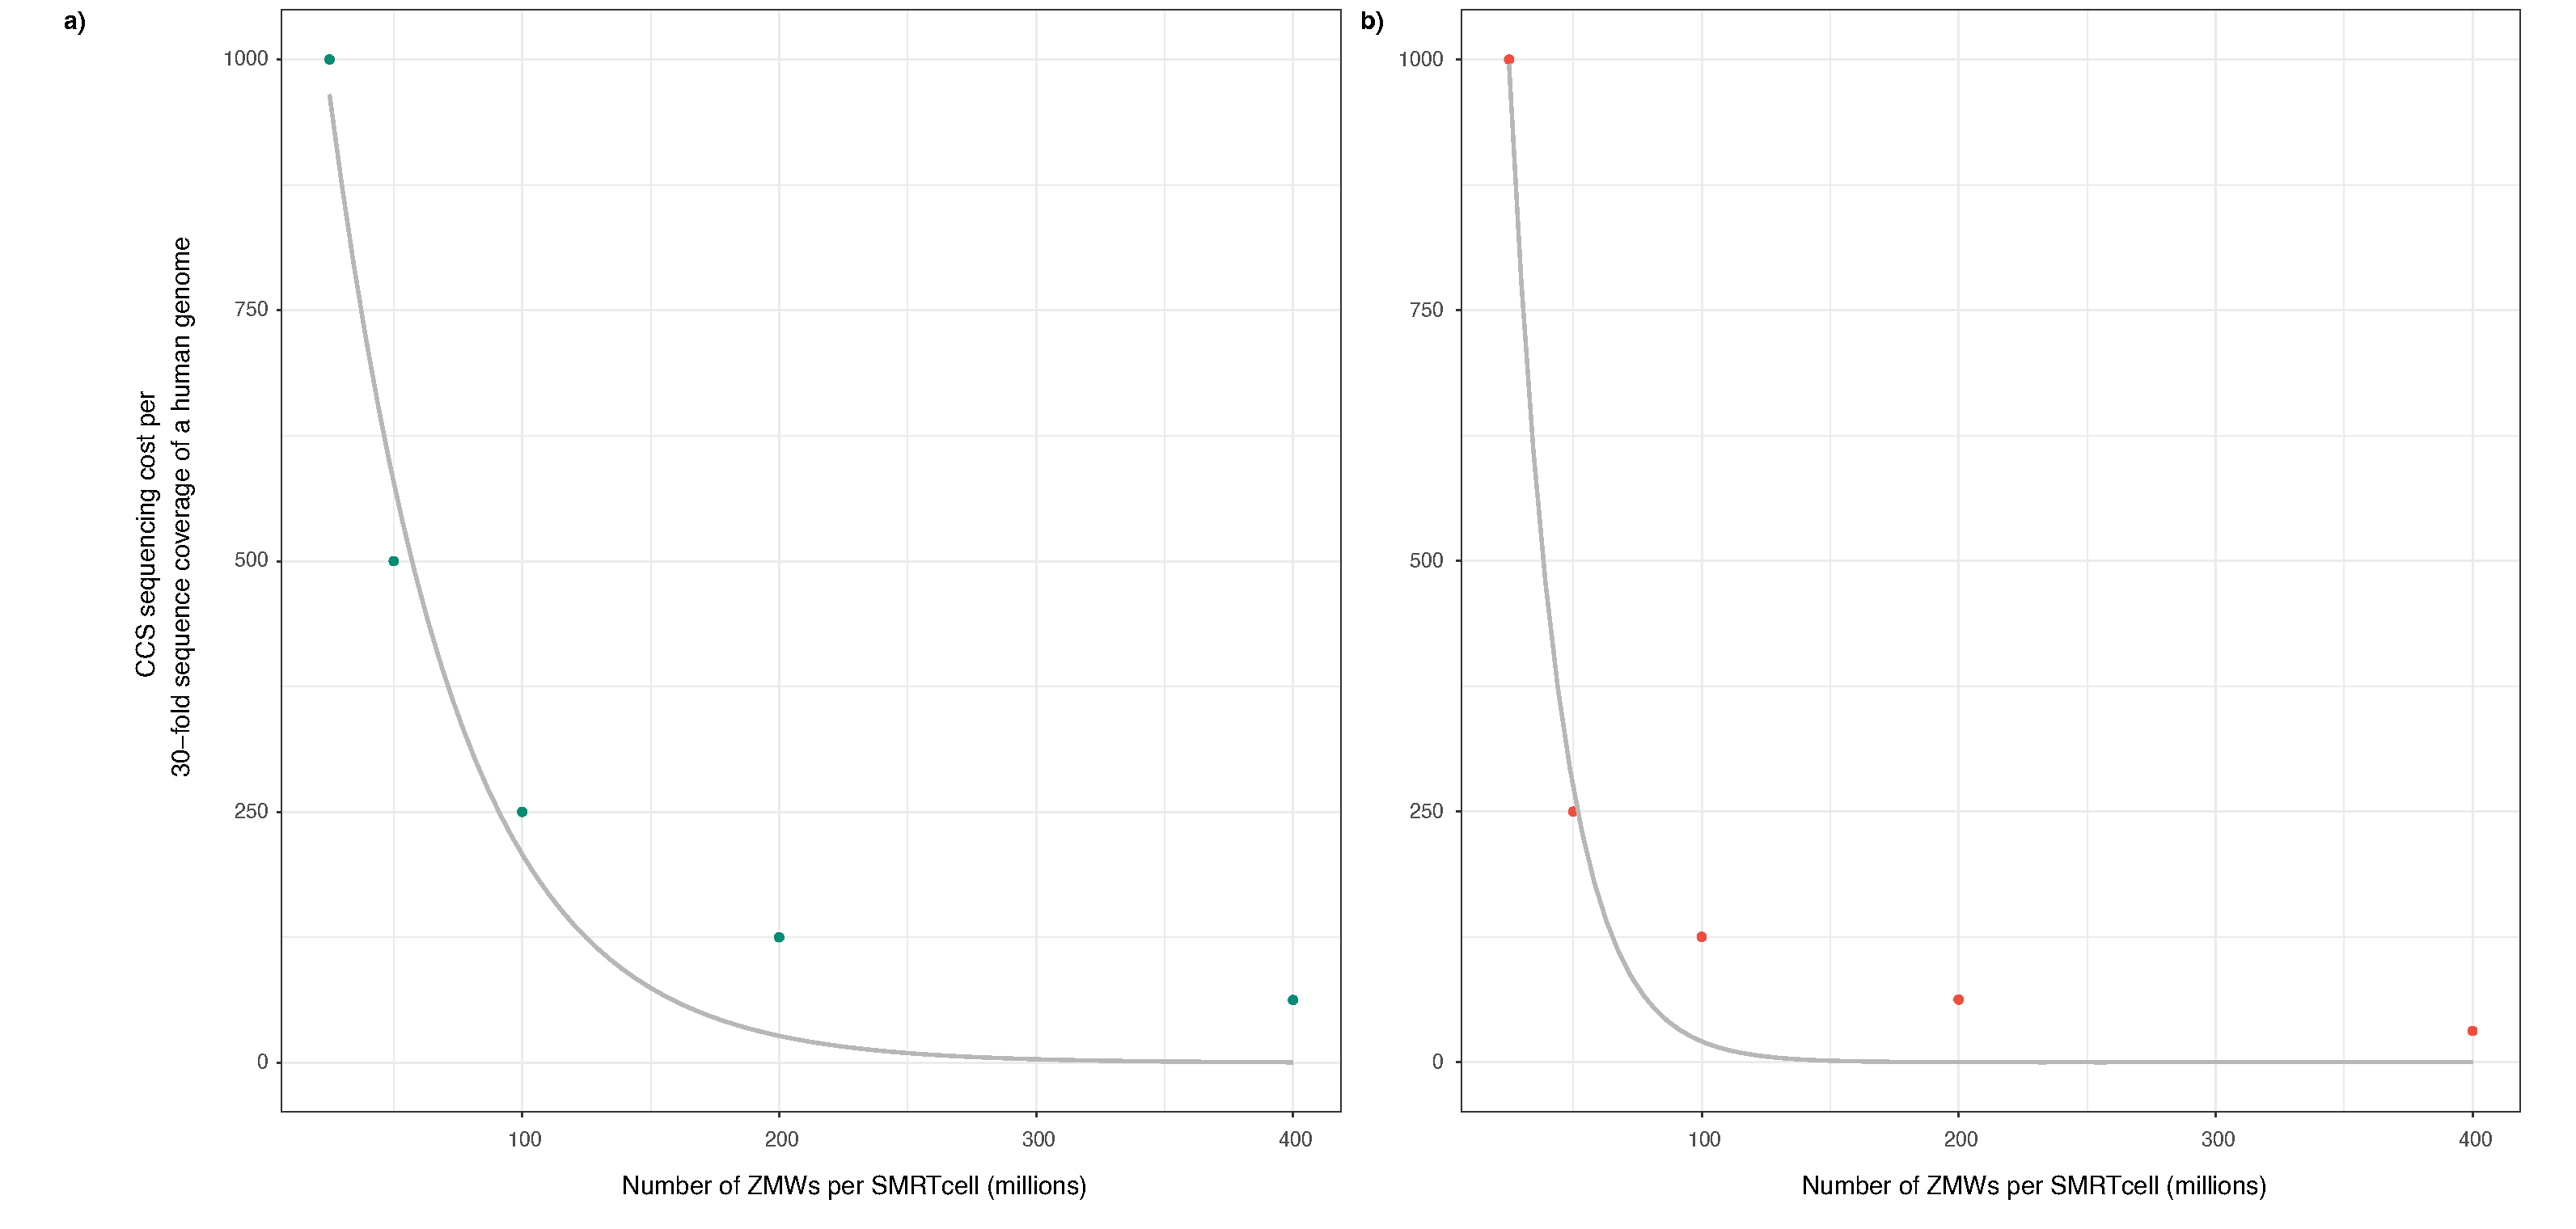
\includegraphics[width=\textwidth]{exponential_decay_in_ccs_sequencing_cost.pdf} \\ \smallskip
\end{centering}
\floatfoot{The graph starts with the current CCS sequencing cost for a 30-fold sequence coverage of a human genome using the Revio instrument, which is based on the latest SMRTcell with 25 million ZMWs and assumes that average CCS read length is around 20kb. \textbf{a)} Exponential decay in CCS sequencing cost with doubling in the number of ZMWs per SMRTcell. \textbf{b)} Exponential decay in CCS sequencing cost with doubling in both CCS read length and the number of ZMWs per SMRTcell.}
\end{figure}

%\begin{figure}[h!]
%\caption{Pacific Biosciences flywheel}
%\label{figure:flywheel}
%\begin{centering}
%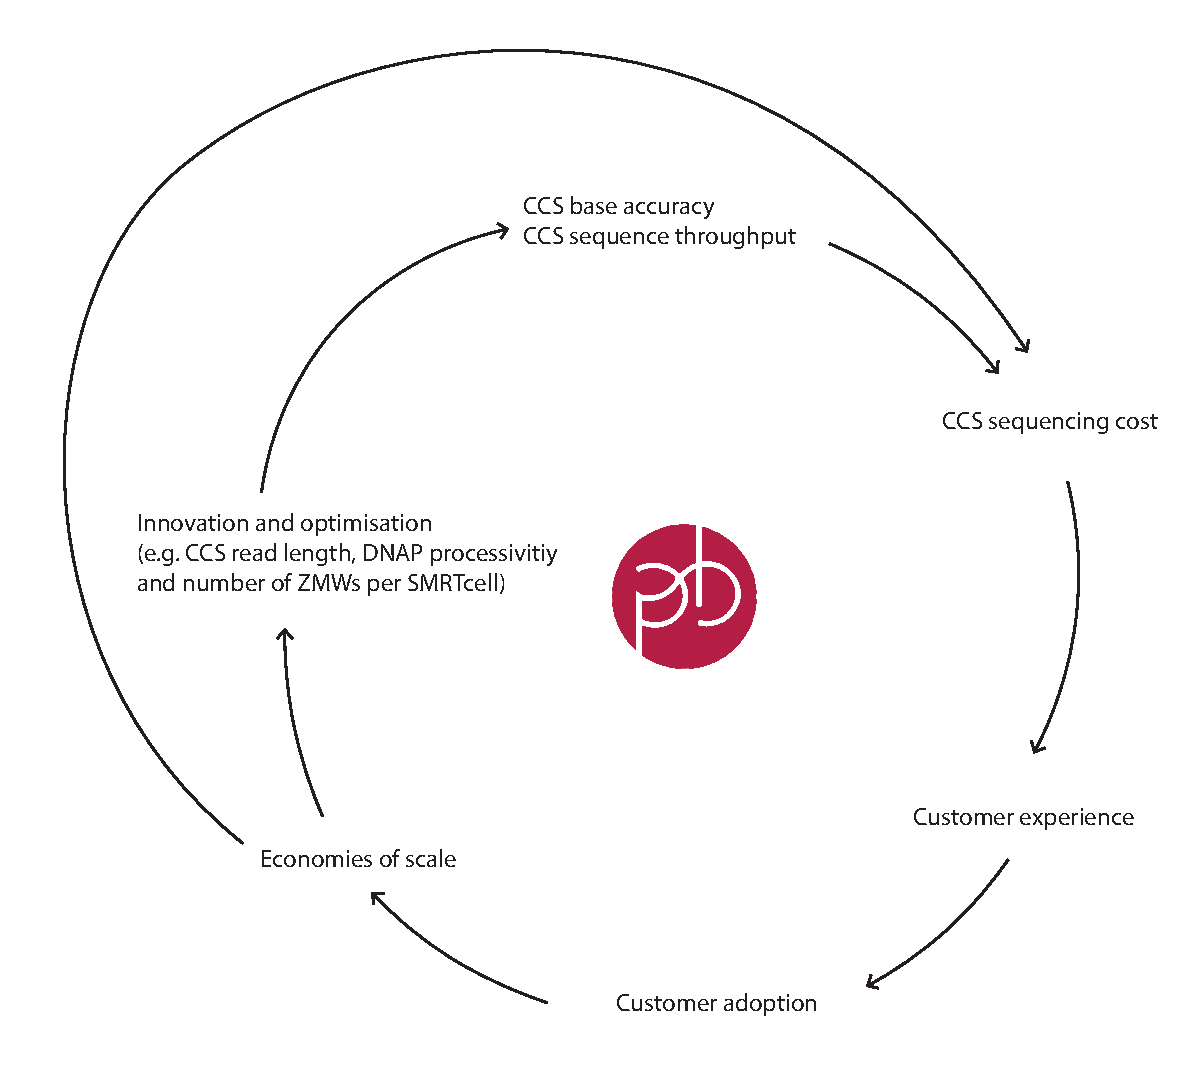
\includegraphics[width=0.75\textwidth]{pacbio_flywheel.pdf} \\ \smallskip
%\end{centering}
%\floatfoot{The flywheel symbolises how independent components act in concert to improve base accuracy, reduce sequencing cost and drive customer adoption}
%\end{figure}

DNAP processivity, which is the rate at which DNAP synthesises a new strand of DNA, is another crucial factor that determines the number of subreads per CCS read. This, in turn, influences CCS sequence throughput and CCS base accuracy. For example, if DNAP processivity is doubled, CCS read length can also be doubled without sacrificing base accuracy. Therefore, the biological limit of DNAP processivity will ultimately determine the CCS read length. 

In the future, I believe that high-throughput SMRT sequencing instruments will produce CCS reads at a fraction of the current costs and that the majority of bases will have base accuracy greater than Q90. Given that CCS reads enables \textit{de novo} assembly and simultaneous detection of haplotype phased somatic and germline mutations as well as base modifications, I believe that CCS sequencing will become the primary DNA sequencing method in the near future. 

\subsection{Strand-specific somatic mutation detection}

To date, somatic mutation detection in normal tissues and tumours with next-generation sequencing has focused on analysing sub-clonal or clonal somatic mutations that are fixed in a group of cells. Single-molecule and strand-specific base modification somatic mutation detection have the potential to enhance our understanding of somatic mutagenesis.

As described in chapter 1 \section{}, DNA polymerase (DNAP) sequences both the forward and reverse strand of the SMRTbell template multiple times through rolling circle sequencing. The pbccs algorithm leverages the redundancies and complementary base pairing between the forward- and reverse-strand subreads to generate CCS reads. As demonstrated in chapter 2, CCS reads have sufficient base accuracy to enable single-molecule somatic mutation detection. Moreover, as described in a previous publication, 5-methylcytosine can be detected in each CCS read using DNAP kinetics \cite{Tse2021-or, Vong2019-bi}. Furthermore, the pbccs algorithm can generate single-strand consensus sequence (SSCS) reads from the forward- and reverse-strand subreads. Strand-specific somatic mutation and base modification detection with SSCS reads present an exciting opportunity to analyse the life cycle of somatic mutations.

Somatic mutation is a three-step process: 1) DNA damage, mutation, or modification from endogenous or exogenous sources, 2) failure to detect and repair the DNA damage or mutation, and 3) the persistence of DNA mutation in daughter cells through genetic drift or selection. In any population of DNA molecules, there will be four groups: 1) there will be a group of wild type DNA molecules with the original template sequence, 2) a group of DNA molecules with DNA damage, mutation, or base modification, 3) a group of DNA molecules undergoing DNA damage repair, and 4) a group of DNA molecules with newly acquired somatic mutations (Fig \ref{figure:single-strand-specific-mutation}). 

\begin{figure}[htbp!]
\caption{SBS1 somatic mutational process}
\label{figure:single-strand-specific-mutation}
\begin{centering}
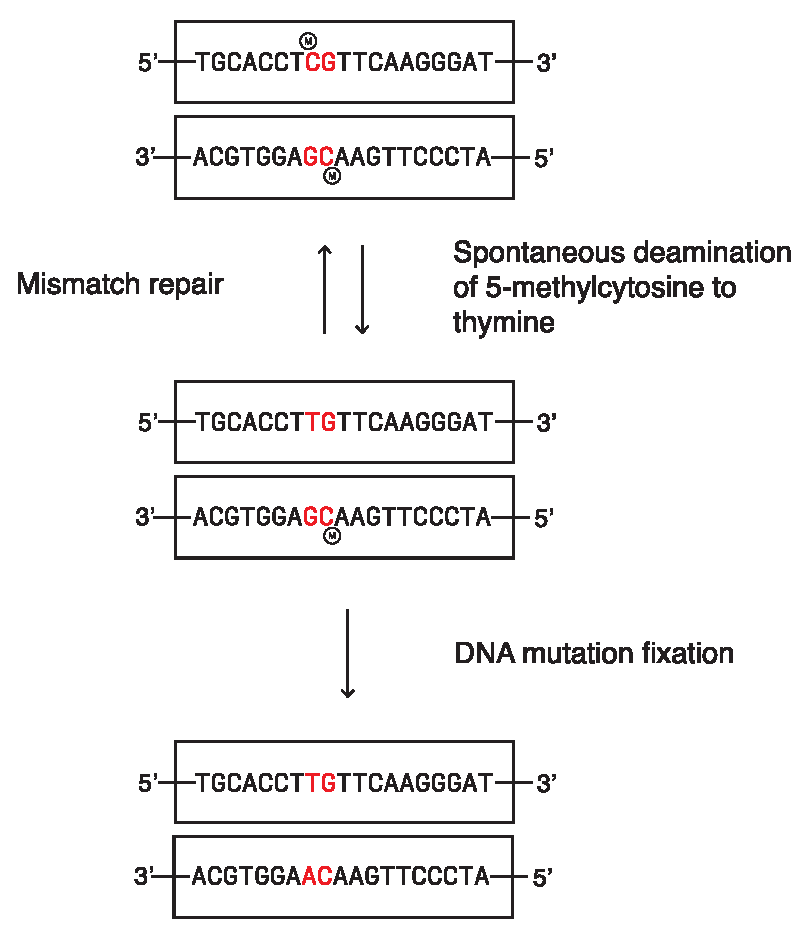
\includegraphics[width=\textwidth]{spontaneous_deamination_horizontal.pdf} 
\end{centering}
\floatfoot{The figure illustrates how DNA mismatch resulting from spontaneous deamination of 5mC to thymine is repaired and how DNA mutation is fixed. The nucleotide bases in red highlights the methylated CG dinucleotide on both the forward and reverse strand of the DNA.}
\end{figure}

For example, the availability of CCS reads, SSCS reads, and the base modifications associated with both datasets facilitates the examination of DNA damage and repair processes associated with the SBS1 mutational signature. The spontaneous deamination of methyl-cytosine to thymine results in a TG:GC mismatch and leads to a C>T substitution at NCG trinucleotide if left unrepaired by the mismatch repair (MMR) pathway. If DNA molecules with damage are sequenced, SSCS reads should enable the successful detection of the TG dinucleotide on the strand where deamination has occurred, while the GC dinucleotide with methylation will be present on the complementary strand (Figure \ref{figure:single-strand-specific-mutation}). CCS reads should also provide an estimate of the number of methylated NCG trinucleotides where deamination can potentially happen, as well as the number of N[C>T]G somatic mutations where deamination has occurred. If the same tissue is sequenced at multiple time points, the gain and loss of somatic mutations could also be studied longitudinally.  

As detailed above, the successful use of SMRT sequencing data will enable the measurement of the \textit{in vivo} deamination rates and comparison to the \textit{in vitro} deamination rate of $5.8\times10^{-13}$ per 5mC per second at 37°C \cite{Shen1994-of}. In addition, TG:GC MMR repair efficiency and fidelity can also be measured under both wild-type and mutant conditions. For example, MutS$\alpha$ is critical in recognising the TG:GC mismatch and initiating DNA damage repair. Individuals with a MutS$\alpha$ deficiency have an elevated number of N[C>T]G somatic mutations. The same approach could also be used to enhance our understanding of APOBEC-dependent deamination of cytosine to uracil, which generates T[C>T]N somatic mutations. 


\subsection{Decomposition of a mutational signature}

Single-molecule resolution and strand-specific base modification somatic mutation detection create an opportunity to gain greater insights into the dynamics of somatic mutational processes. Each somatic mutational process leaves a characteristic imprint to the genome, and mutational signatures represent the probability that a specific mutational process will produce a mutation in a specific sequence context. Each mutational signature results from the cumulative effects of DNA damage, mutations, or base modifications, failures in DNA repair or mismatch correction, and the presence of these mutation in bulk tissue. The method described above should allow us to decompose mutational signature into individual components representing DNA damage, repair and fixation, and to investigate the dynamics between these components. 

% Single-molecule resolution and strand-specific base modification somatic mutation detection create an opportunity to gain greater insights into the dynamics of somatic mutational processes. Each somatic mutational process leaves a characteristic imprint to the genome, and mutational signatures represent the probability that a specific mutational process will produce a mutation in a specific sequence context. Each mutational signature results from the cumulative effects of DNA damage, mutations, or base modifications, failures in DNA repair or mismatch correction, and the presence of these mutation in bulk tissue. The method described above should allow us to decompose mutational signature into individual components representing DNA damage, repair and fixation, and to investigate the dynamics between these components. 

\subsection{Crossover and non-crossover detection using CCS reads}

Here, I hypothesise that CCS read length and base accuracy can be leveraged to gene conversion and crossover (CO) events resulting from meiotic and mitotic recombination.  Gene conversion and CO (Fig \ref{figure:homologous-recombination}) arise from the non-reciprocal and reciprocal exchange of genetic material during double-strand break (DSB) repair. In the literature, gene conversion is also referred to as non-crossover (NCO), but CO and NCO are not mutually exclusive events, as the names suggest \cite{Hunter2015-gk}. 

\begin{figure}[htbp!]
\caption{Gene conversion and crossover}
\label{figure:homologous-recombination}
\begin{centering}
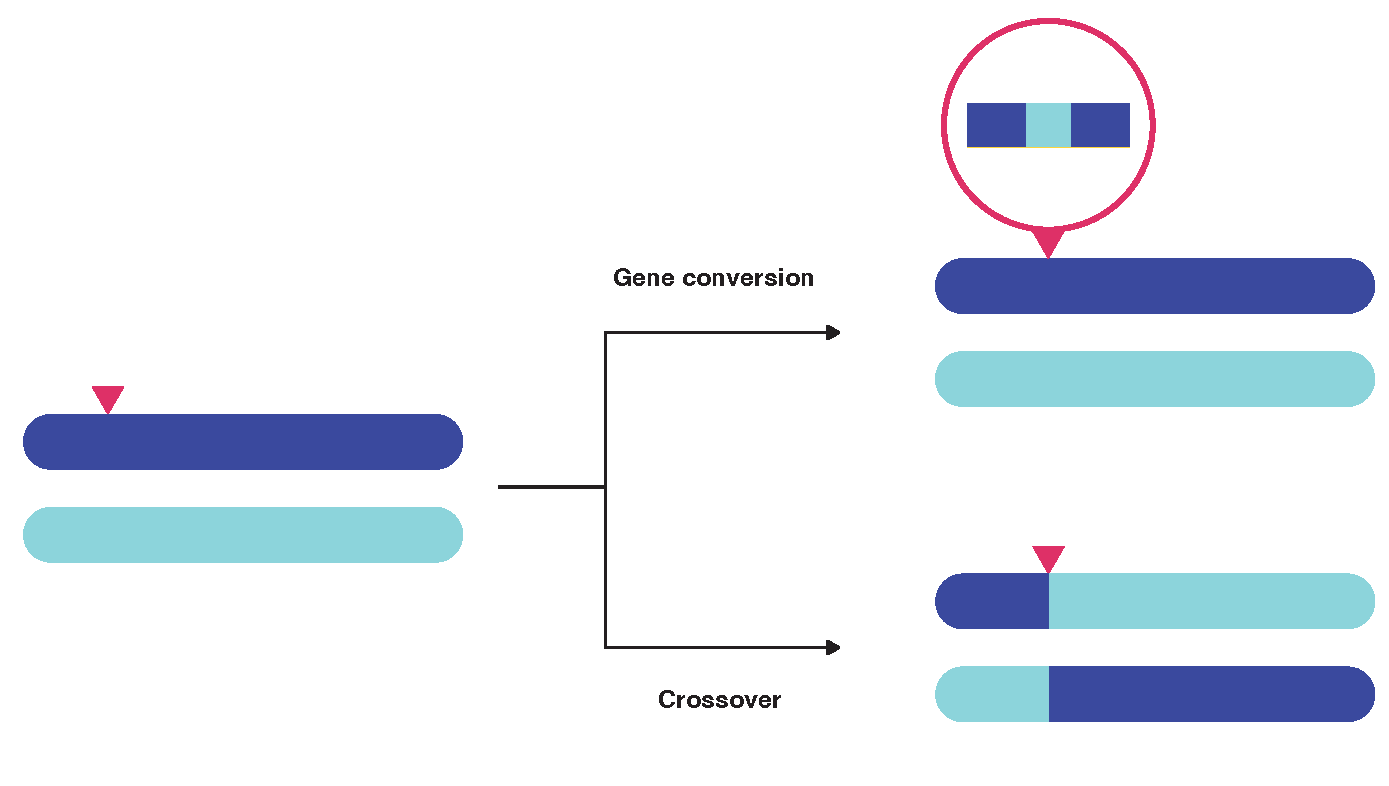
\includegraphics[width=\textwidth]{meiotic_recombination.pdf}
\end{centering}
\floatfoot{Red triangle indicates the DSB site. DSB can be repaired either as a gene conversion or as a crossover. Sister chromatids are not shown for simplification purposes.}
\end{figure}

\subsubsection{Meiotic and mitotic recombination}

In germ cells, meiotic recombination produces new combination of haplotypes, increasing genetic diversity and phenotypic diversity in sexually producing species. This diversity is the basis for adaptation and speciation through natural selection and sexual selection. In addition, meiotic recombination also ensures the proper segregation of sister chromatids through the formation of at least one chiasma per pair of homologous chromosomes during anaphase I of meiosis. Improper segregation of sister chromatids can result in aneuploid gametes with abnormal number of chromosomes, leading to developmental disorders or miscarriages. 

In somatic cells, successful mitotic recombination leads to copy number neutral (CNN) loss of heterozygosity (LOH), where the exchange of genetic material results in the replacement of one copy of parental DNA, leading to homozygosity at the site of exchange \cite{}. In contrast to meiotic recombination, where an individual might gain a selective advantage compared to other individuals in a population, mitotic recombination can confer proliferative advantage to a cell and contribute to tumorigenesis. In addition, one of the main differences between meiotic and mitotic recombination is that in germ cells, the induction of DSB is programmed, whereas in somatic cells, DSBs are introduced as a result DNA damage from endogenous (e.g., reactive oxygen species) and exogenous (e.g., ionising radiation) factors \cite{}. 

\subsubsection{Existing methods for detecting meiotic recombination}

In principle, detecting gene conversion and crossover requires determining the original parental haplotype and comparing it to the new haplotype produced by meiotic recombination to identify the site of genetic material exchange. Here, a haplotype is defined as a set of alleles located on the same physical chromosome. To date, trio-sequencing \cite{Kong2010-uk}, sperm-typing \cite{Webb2008-pw} and statistical methods leveraging the non-random association of alleles (linkage disequilibrium) \cite{Myers2005-ml} have been primarily used to study human meiotic recombination. Each method has trade-offs in the resolution and the number of meiotic recombination events detected. The resolution of meiotic recombination events depends on the heterozygosity of the individual, the density of genetic markers, and the distance between the genetic markers where meiotic recombination has been detected \cite{}. 

With whole-genome sequence data from a child, both biological parents, and grandparents, chromosome-scale haplotypes of both the child and parents can be obtained through haplotype phasing. Afterwards, gene conversion and crossover are detected by comparing the child’s haplotype and the parents’ haplotype. The trio-sequencing approach detects at least one meiotic recombination per chromosome per child, and the number of detected meiotic recombination events scales with the number of children sequenced. In addition, unlike other approaches, the trio-sequencing approach enables the examination of meiotic recombination dynamics, such as crossover interference \cite{} and the study of sex-specific meiotic recombination \cite{}. 

As an alternative to pedigree analysis, sperm-typing compares haplotypes between sperm cells obtained from the same individual to analyse recombinant and non-recombinant DNA molecules at previously established meiotic recombination hotspots. Using allele-specific PCR primers, DNA segments containing two or more polymorphic markers are amplified to capture DNA molecules from a specific meiotic recombination hotspot. Afterwards, DNA segments from individual sperm cells are compared to determine the haplotype and identify recombinant and non-recombinant molecules \cite{}. A major advantage of sperm-typing over existing methods is that the sample size is practically unlimited, given that millions of sperm cells are produced daily and are present in semen. This allows for the study of a large number of meioses. Consequently, in contrast to other methods, sperm-typing can directly count the number of recombinant and non-recombinant molecules, measure recombination frequencies, and calculate the CO to NCO ratio \cite{}. As a result, sperm-typing enables the most detailed examination of individual meiotic recombination hotspots. To date, sperm-typing has been used to estimate gene conversion tract length \cite{}, calculate recombination frequencies across different meiotic recombination hotspots \cite{}, and study inter-individual variations in recombination outcomes \cite{}. 

Finally, statistical methods use polymorphism data from unrelated individuals and unobserved recombination in previous generations to infer recombination rates and to generate high-resolution recombination maps. These methods leverage linkage disequilibrium (LD), defined as the non-random association between alleles at different loci in a breeding population, and the disruption of LD through recombination to estimate recombination rate between loci. As expected, loci that are close to each other are rarely separated by recombination, while recombination occurs frequently between distant loci.  Therefore, LD provides information about not only the recombination rate, but also the number of generations of recombination. Statistical methods have several limitations. One limitation is the inability to examine inter-individual and intra-individual variations in meiotic recombination. Another limitation is that these methods provide an averaged recombination rate across sexes, time, and the whole population. 

\subsubsection{Meiotic recombination detection using CCS reads}

Here, I hypothesise that CCS sequencing will enable genome-wide detection of meiotic and mitotic recombination in bulk sperm and bulk normal tissue sample, respectively. At a locus where meiotic or mitotic recombination has occurred, there will be three groups of CCS reads: those derived from the maternal haplotype, those derived from the paternal haplotype, and those containing both maternal and paternal haplotypes. A hypothetical method would leverage CCS read length to haplotype-phased the genome. Afterwards, CCS reads would be compared against the consensus haplotype to identify CCS reads with non-consensus haplotypes. The length and the number of phase transitions, defined as changes from the maternal allele to the paternal allele and vice versa, will determine whether the recombination is classified as a gene conversion or crossover.  Typically, gene conversions measure 300 to 500bp in length, exhibit one phase transition \cite{}. On the other hand, crossovers result in phase transitions at all heterozygous mutations downstream of the meiotic recombination site. 

\begin{figure}[h!]
\caption{Gene conversion and crossover detection using CCS reads}
\label{figure:phase-transitions}
\begin{centering}
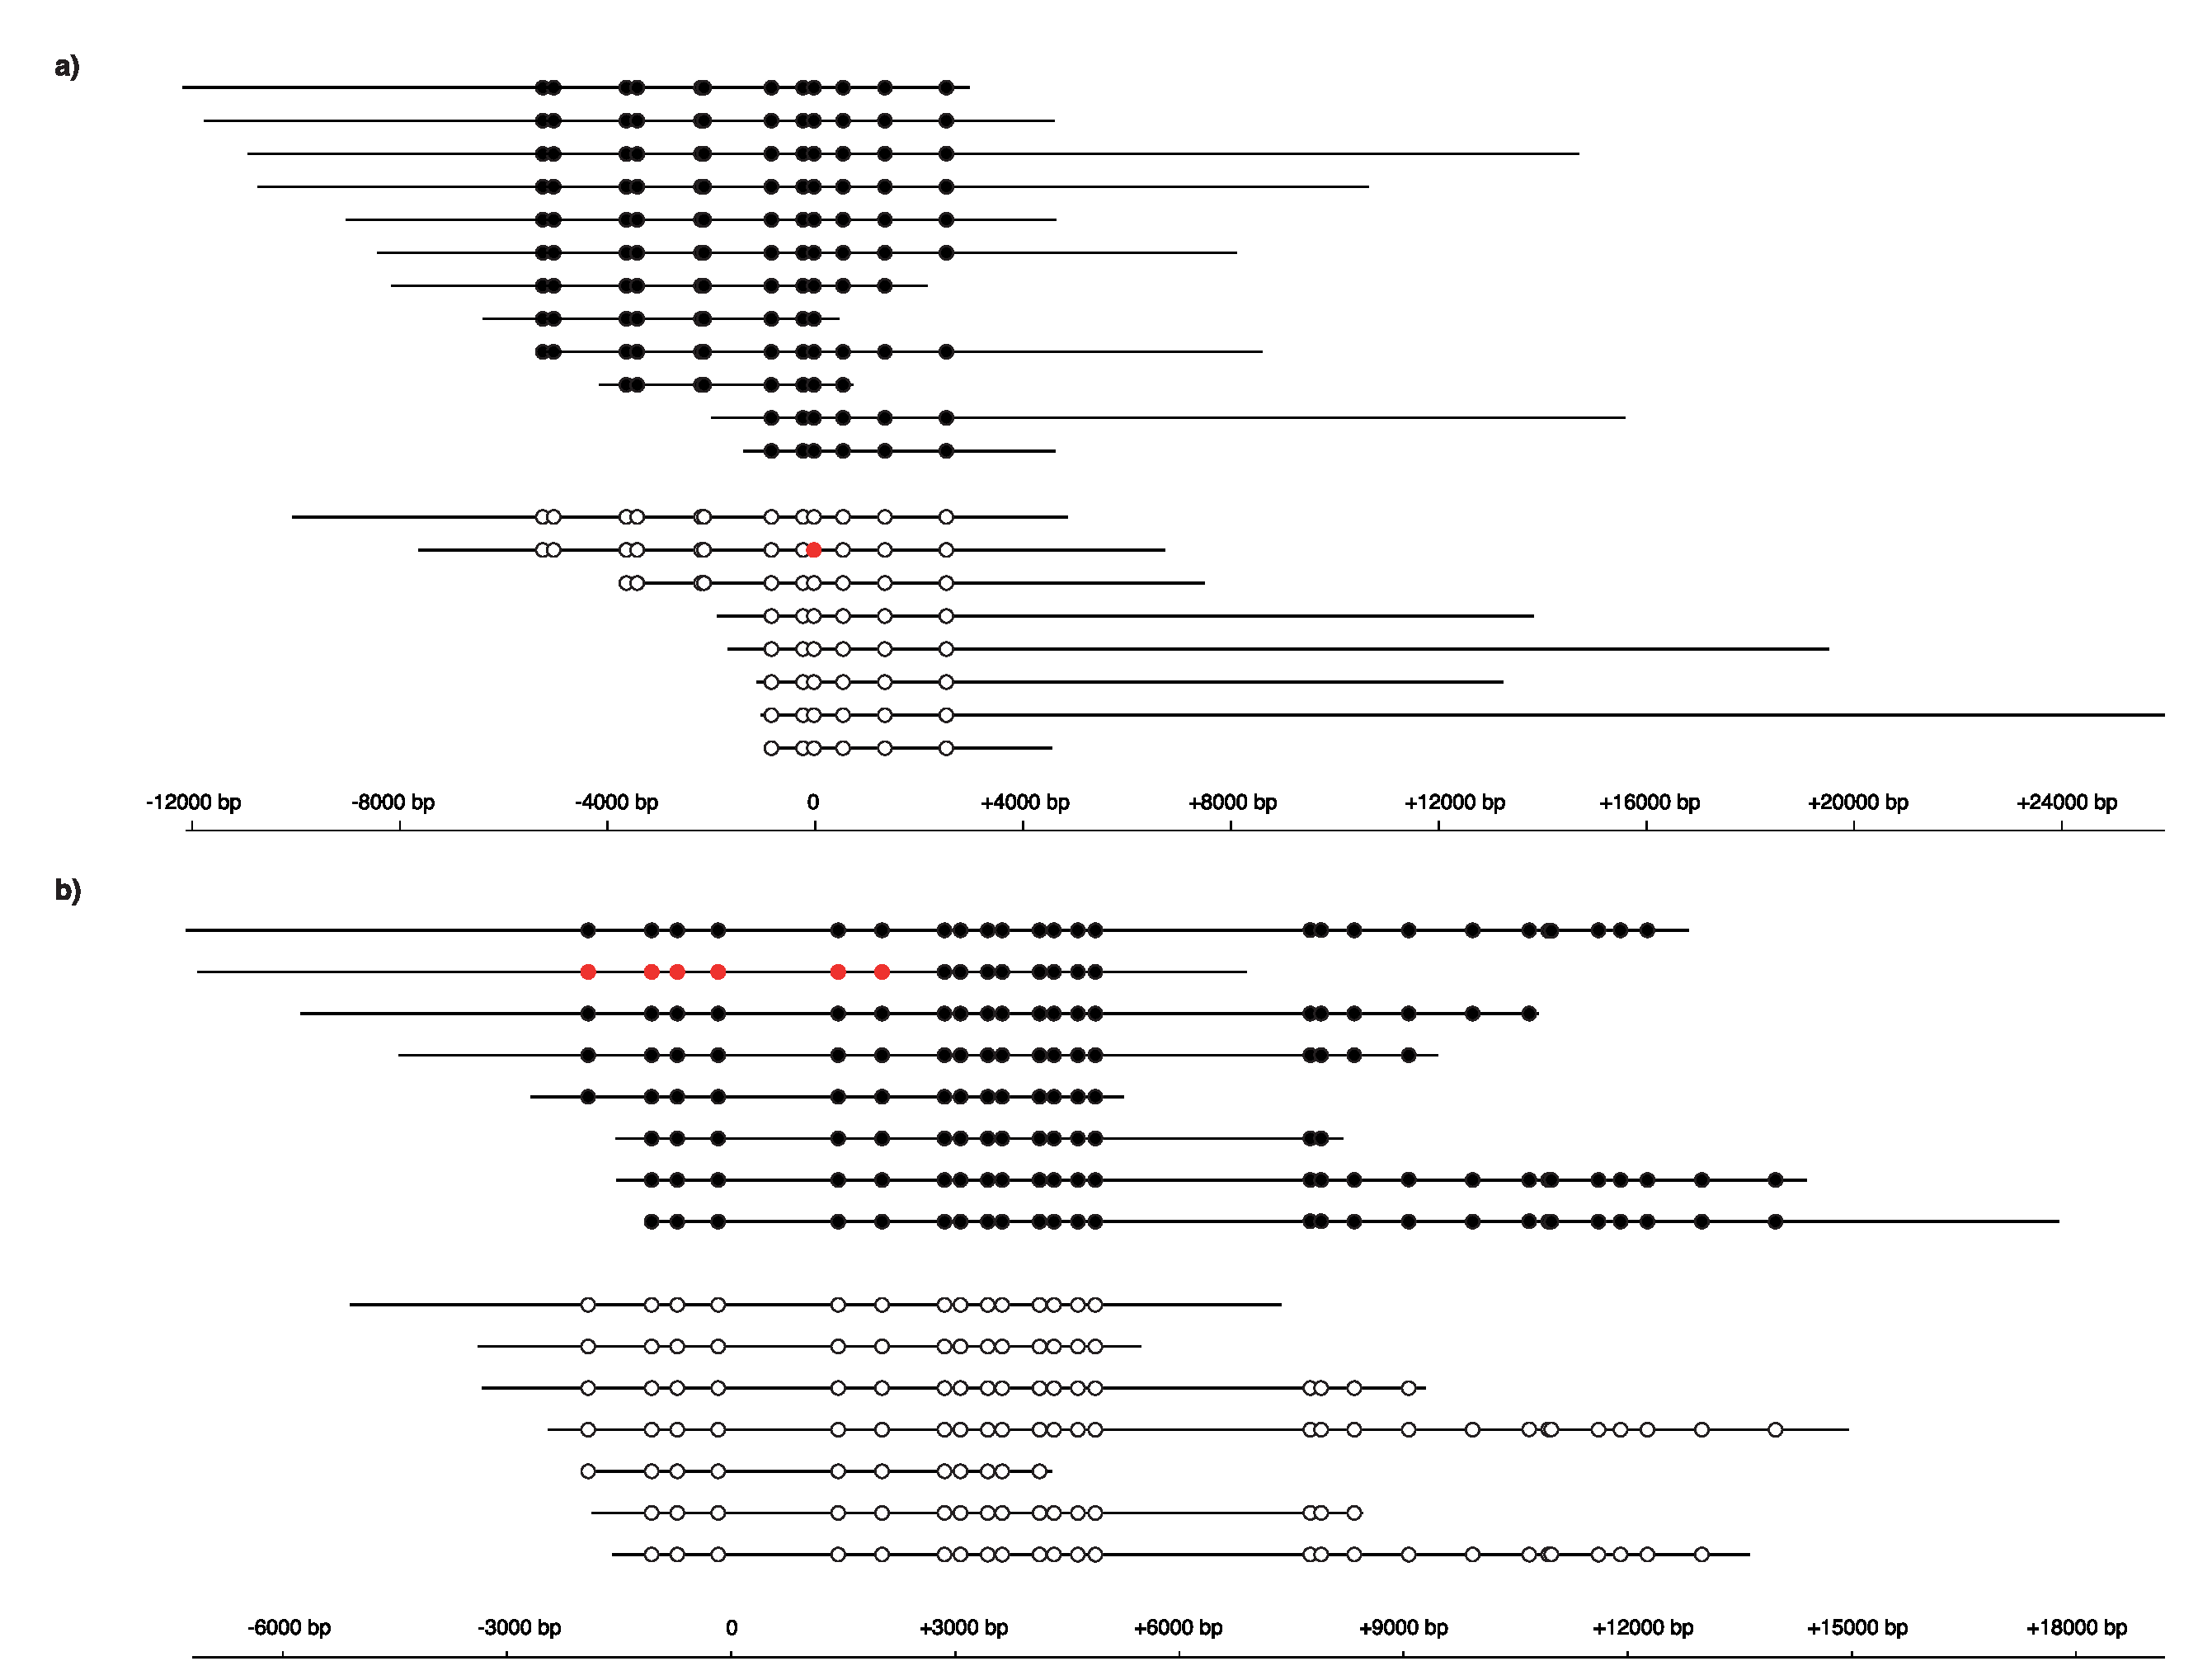
\includegraphics[width=\textwidth]{meiotic_recombination_detection.pdf} 
\end{centering}
\floatfoot{Each circle indicates a heterozygous SNP. A black circle indicates a reference allele, white circle indicates an alternative allele and red circle indicates a phase transition from reference allele to alternative allele and vice versa. CCS reads derived from the same haplotype have the same set of heterozygous SNPs. \textbf{a)} Gene conversion detection using CCS reads requires the phase transition to be flanked by wild type alleles of the haplotype. \textbf{b)} Crossover detection using CCS reads necessitates the phase transition to be continuous.}
\end{figure}

Before I detail how advantages and disadvantages of the hypothetical method in specific applications, I would like to call attention to one major difference between detection of meiotic and mitotic recombination. Meiosis, through two rounds of cell divisions, produce four gametes. Of the four gametes, two will have the original haplotype, whereas the other two will have recombinant haplotypes specific to each gamete. In other words, each recombinant haplotype produced through meiotic recombination is unique and cannot be observed more than once. In addition, because at least one chiasma per pair of homologous chromosomes is required for proper segregation of sister chromatids during meiosis, the number of detected meiotic recombination events is proportional to sequence coverage. In contrast, while mitotic recombination might occur in a single cell, if the LOH generated through mitotic recombination confers a proliferative advantage, the affected cell can outcompete neighbouring cells and expand to occupy larger areas of the tissue. Consequently, the mitotic recombination will be detected in more than one read.

Compared to existing methods, detection of meiotic recombination using CCS reads has several advantages and may enhance our understanding of biological mechanisms behind meiotic recombination. For example, while sperm-typing is limited to previously identified meiotic recombination hotspots, bulk sperm CCS sequencing allows for genome-wide detection of meiotic recombination and the subsequent construction of individual genome-wide recombination maps. In addition, as discussed in chapter 2, CCS reads can be used to profile ongoing somatic mutational processes in bulk normal tissue. Similarly, CCS reads can also be used to profile ongoing \textit{de novo} mutational processes in bulk sperm samples. Currently, the primary mutational processes in germline cells are determined to be spontaneous deamination of methyl-cytosine to thymine (SBS1) and a cell-division independent mutational process (SBS5) \cite{}.  Additionally, while a mutational process associated with CO has been identified \cite{}, to my knowledge, mutational process associated with NCO has not been examined in detail. In short, CCS reads could enable both meiotic recombination and \textit{de novo} mutation detection. 

% Compared to existing methods, detection of meiotic recombination using CCS reads has several advantages and may enhance our understanding of biological mechanisms behind meiotic recombination. For example, while sperm-typing is limited to previously identified meiotic recombination hotspots, bulk sperm CCS sequencing allows for genome-wide detection of meiotic recombination and the subsequent construction of individual genome-wide recombination maps. In addition, as discussed in chapter 2 \section{}, CCS reads can be used to profile ongoing somatic mutational processes in bulk normal tissue. Similarly, CCS reads can also be used to profile ongoing \textit{de novo} mutational processes in bulk sperm samples. Currently, the primary mutational processes in germline cells are determined to be spontaneous deamination of methyl-cytosine to thymine (SBS1) and a cell-division independent mutational process (SBS5) \cite{}.  Additionally, while a mutational process associated with CO has been identified \cite{}, to my knowledge, mutational process associated with NCO has not been examined in detail. In short, CCS reads could enable both meiotic recombination and \textit{de novo} mutation detection. 

The PRDM9 gene plays an essential role in the initiation of meiotic recombination \cite{}.  PRDM9 binds to a specific DNA sequence motif (CCNCCNTNNCCNC) \cite{Myers2008-st}, catalyses the transfer of methyl groups to histone proteins as a methyltransferase \cite{} to make the DNA more accessible to proteins, and recruits SPO11 for programmed induction of DSBs. The PRDM9 zinc finger array determines the sequence motif of PRDM9 binding sites and, consequently, the location of meiotic recombination hotspots. The ability to determine the PRDM9 allele and to detect genome-wide \textit{de novo} mutations and meiotic recombination using CCS reads might facilitate the examination of inter-individual and intra-individual variation in meiotic recombination. Moreover, single-cell whole-genome amplification can be performed to study meiotic chromosome dynamics, complementing areas of meiotic recombination biology that bulk sperm CCS sequencing alone cannot address


\section{Concluding remarks}

In this PhD thesis, I introduce a method to detect single-molecule somatic mutations from PacBio CCS reads and apply it to study germline and somatic mutational processes across the Tree of Life. To demonstrate that CCS bases have sufficient base accuracy for profiling ongoing somatic mutational processes in normal human tissue, I develop a unique benchmarking to unbiasedly assess the sensitivity for detecting somatic mutations randomly distributed across the genome. My analysis indicates that the CCS sequencing error rate is higher than the human somatic mutation rate. However, since the number of sequencing errors is lower or comparable to the number of somatic mutations found in typical adult normal tissue, somatic mutation detection using CCS reads enables the profiling of ongoing somatic mutational processes across a diverse range of eukaryotic species. 

In the future, I believe that PacBio will be able to exponentially improve CCS sequence throughput and reduce the CCS sequencing error rate below the human somatic mutation rate. As discussed in chapters 1 and 2, read-of-insert length, DNAP processivity and the number of ZMWs per SMRTCell determines CCS sequence throughput. PacBio has continually improved these factors to reduce the per-base sequencing cost, and further advances are expected to be in the pipeline. Above all, my research indicates that inaccurate BQ score estimation, rather than CCS library preparation and SMRT sequencing, is the source of false positive somatic mutations, and that more accurate CCS bases can be obtained with updates to the consensus sequence algorithm. I believe that we are witnessing a historic moment in which nearly error-free sequencing will be possible at a fraction of current costs, allowing us to interrogate the genetic, epigenetic, and transcriptomic information of all forms of life, and transform our understanding of life. 









